\documentclass[aspectratio=169]{beamer}


% Beamer settings
\usecolortheme{rose}
\beamertemplatenavigationsymbolsempty
\setbeamertemplate{footline}[frame number]

\titlegraphic{%

\includegraphics[height=1cm]{logo-full-colour.png}}

\addtobeamertemplate{frametitle}{}{%
\begin{tikzpicture}[remember picture,overlay]
\node[anchor=north east,yshift=2pt] at (current page.north east) {
\includegraphics[height=1cm]{logo-full-colour.png}};
\end{tikzpicture}}

% Packages
\usepackage{amsmath}

\usepackage{tikz}
\usetikzlibrary{positioning}
\usetikzlibrary{fit}

\usepackage{pgfplots}
\usepgfplotslibrary{fillbetween}

\usepackage{minted}
\usepackage[T1]{fontenc} % Required by minted to ensure dollar signs are produced instead of pound (sterling) signs

\usepackage{multicol}

\usepackage{booktabs}

\usepackage{adjustbox}

% Author
\author{Simon McIntosh-Smith \& Tom Deakin\\University of Bristol}

\date{}



\title{OpenMP for Computational Scientists}
\subtitle{3: Vectorisation and NUMA}

\begin{document}

\frame{\titlepage}

%-------------------------------------------------------------------------------
\begin{frame}[fragile]
\frametitle{Previous exercise}

Take your parallel 5-point stencil, and implement a reduction:
\begin{minted}[frame=single,breaklines,fontsize=\small]{fortran}
total = 0.0
!$omp parallel do collapse(2) reduction(+:total)
do i = 1, nx
    do j = 1, ny
    Atmp(i,j) = (A(i-1,j) + A(i+1,j) + A(i,j) + A(i,j-1) + A(i,j+1)) / 5.0
    total = total + Atmp(i,j)
    end do
end do
!$omp end parallel do
\end{minted}

\begin{itemize}
    \item Well done if you managed this!
    \item 5-point stencil is simple, but captures the \emph{essence} of more complicated codes.
    \item Extension: did anyone try the parallelising the Jacobi solver?
\end{itemize}

\end{frame}

%-------------------------------------------------------------------------------
%-------------------------------------------------------------------------------
\section{Vectorisation}
\begin{frame}
\frametitle{Vectorisation}
$$C=A+B$$
\begin{columns}
\begin{column}{0.5\textwidth}
Scalar operations \\
\begin{adjustbox}{max totalsize={\textwidth}{0.6\textheight},center}

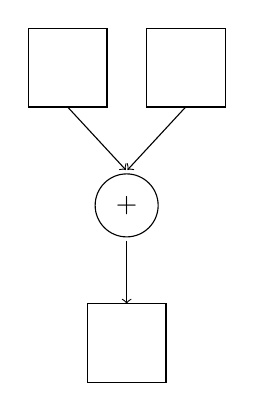
\begin{tikzpicture}
  \draw (-0.5,2) rectangle (0.5,3);
  \draw (1,2) rectangle (2,3);
  \draw[->] (0,2) -- (.74,1.2);
  \draw[->] (1.5,2) -- (.76,1.2);
  \draw (.75,.75) circle (.4cm);
  \draw (.75,.75) node {$+$};
  \draw[->] (.75,0.3) -- (.75,-0.5);
  \draw (.25,-1.5) rectangle (1.25,-0.5);
\end{tikzpicture}
\end{adjustbox}
\end{column}

\begin{column}{0.5\textwidth}
Vector operations \\
\begin{adjustbox}{max totalsize={\textwidth}{0.6\textheight},center}
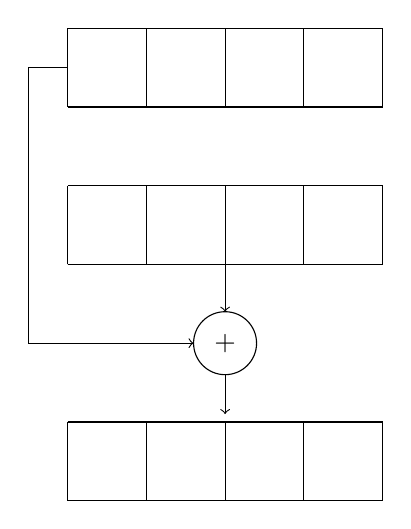
\begin{tikzpicture}
  \draw[step=1cm] (0,2) grid (4,3);
  \draw[step=1cm] (0,0) grid (4,1);
  \draw[->] (2,0) -- (2,-0.6);
  \draw[->] (0,2.5) -- (-0.5,2.5) -- (-0.5,-1) -- (1.6,-1);
  \draw (2,-1) circle (.4cm);
  \draw (2,-1) node {$+$};
  \draw[->] (2,-1.4) -- (2,-1.9);
  \draw[step=1cm] (0,-3) grid (4,-2);
\end{tikzpicture}
\end{adjustbox}
\end{column}
\end{columns}

\end{frame}

%-------------------------------------------------------------------------------
\begin{frame}
\frametitle{Why vectorise?}
\begin{itemize}
  \item Vectorisation gives you more compute per cycle.
  \item Hence may increase the FLOP/s rate of the processor.
  \item Also results in fewer instructions to process (less pressure on instruction decode units).
  \item Vectors help make good use of the memory hierarchy (often the main benefit).
  \item Vectorisation helps you write code which has good access patterns to maximise bandwidth.
\end{itemize}
\end{frame}

%-------------------------------------------------------------------------------
\begin{frame}
\frametitle{Auto-vectorisation}
\begin{itemize}
  \item Modern compilers are very good at automatically vectorising your loops.
  \item Fortran helps as arrays can not alias (overlap), unlike C.
  \item But compiler needs to be sure it's safe to vectorise.
  \item Read compiler reports to see if it's already vectorising.
    \begin{itemize}
      \item Intel: \mintinline{bash}|-qopt-report=5|
      \item Cray: \mintinline{bash}|-hlist=a|
      \item GNU (old): \mintinline{bash}|-ftree-vectorizer-verbose=2|
      \item GNU (new): \mintinline{bash}|-fopt-info-vec|
      \item Clang: \mintinline{bash}|-Rpass=loop-vectorize| \mintinline{bash}|-Rpass-missed=loop-vectorize| \mintinline{bash}|-Rpass-analysis=loop-vectorize|
    \end{itemize}
  \item Often the memory access pattern prevents (efficient) auto-vectorisation.
\end{itemize}
\end{frame}

%-------------------------------------------------------------------------------
\subsection{OpenMP SIMD}
\begin{frame}[fragile]
\frametitle{OpenMP SIMD}
\begin{itemize}
  \item Sometimes the compiler needs help in confirming loops are vectorisable.
  \item OpenMP \mintinline{fortran}|simd| constructs give this information.
  \item Can combine with \mintinline{fortran}|parallel do| construct to ensure a parallel vector loop: \mintinline{fortran}|omp parallel do simd|
  \item Generally want to vectorise inner loops and parallelise outer loops.
\end{itemize}

\begin{minted}[frame=single]{fortran}
!$omp simd
do i = 1, N
  C(i) = A(i)+B(i)
end do
!$omp end simd
\end{minted}
\end{frame}

%-------------------------------------------------------------------------------
\begin{frame}[fragile]
\frametitle{SIMD functions}
Say you've written an update function to update values in the loop:
\begin{minted}[frame=single]{fortran}
do i = 1, N
  A(i) = magic_maths(A(i))
end do
\end{minted}

\begin{itemize}
  \item The situation gets complicated.
  \item If the function is small, then likely inlined and loop will auto-vectorise.
  \item Otherwise need to use the \mintinline{fortran}|simd| construct, but need compiler to create a vector version of the function.
\end{itemize}

\begin{minted}[frame=single]{fortran}
function magic_maths(value) result(r)
!$omp declare simd(magic_maths)
  implicit none
  real(kind=8) :: value, r
  r = value * value
end function
\end{minted}

\end{frame}

%-------------------------------------------------------------------------------
\begin{frame}[fragile]
\frametitle{SIMD clauses}
\begin{itemize}
  \item All the usual data-sharing and reduction clauses can be applied.
  \item \mintinline{fortran}|safelen(4)|: distance between iterations where its safe to vectorise.
  \begin{minted}[frame=single]{fortran}
  !$omp simd safelen(4)
  do i = 1, N-4
    A(i) = A(i) + A(i+4)
  end do
  !$omp end simd
  \end{minted}
  \item \mintinline{fortran}|simdlen(4)|: preferred iterations to be performed concurrently as a vector.
  Specifying explicit vector lengths builds in obsolescence to the code as hardware vector lenghts continually change --- don't recommend using this clause.
\end{itemize}
\end{frame}

%-------------------------------------------------------------------------------
\begin{frame}[fragile]
\frametitle{SIMD clauses}
\begin{itemize}
  \item \mintinline{fortran}|linear(var)|: variable is private and linear to the loop iterator.
  \begin{minted}[frame=single]{fortran}
  !$omp simd linear(j)
  do i = 1, N
    j = j + 1
    A(j) = B(i)
  end do
  !$omp end simd
  \end{minted}
  \item \mintinline{fortran}|aligned(var)|: says the array is aligned.
  \item \mintinline{fortran}|uniform(var)|: for \mintinline{fortran}|declare simd| construct, the variable is the same in all vector lanes.
\end{itemize}
\end{frame}

%-------------------------------------------------------------------------------
\begin{frame}
\frametitle{SIMD summary}

\begin{itemize}
  \item Sometimes need to force the compiler to auto-vectorise (the correct) loop with the \mintinline{fortran}|simd| construct.
  \item As with \mintinline{fortran}|parallel|, you are telling the compiler it is safe to vectorise and to ignore its data dependancy analysis.
  \item Check the compiler report before and after the check it did the right thing!
  \item Use \mintinline{fortran}|declare simd| and appropriate clauses if you need to create vectorised versions of functions.
  \begin{itemize}
    \item The clauses can give more information to the compiler so it does a better job.
  \end{itemize}
\end{itemize}

\end{frame}

%-------------------------------------------------------------------------------
\section{Derived types}
\begin{frame}[fragile]
\frametitle{Derived types}
2D grid of cells, each cell containing 4 different values.
\begin{minted}[frame=single,linenos,fontsize=\footnotesize]{fortran}
type cell
  real(kind=8) :: property1
  real(kind=8) :: property2
  real(kind=8) :: property3
  real(kind=8) :: property4
end type

type(cell), allocatable :: grid(:,:)

do j = 1, ny
  do i = 1, nx
    grid(i,j)%property1 = update_1()
    grid(i,j)%property2 = update_2()
    grid(i,j)%property3 = update_3()
    grid(i,j)%property4 = update_4()
  end do
end do
\end{minted}
\end{frame}

%-------------------------------------------------------------------------------
\begin{frame}
\frametitle{Derived types}
\begin{itemize}
  \item What do Fortran derived types look like in memory?
  \item Organised as an array of structures.
  \item<2-> What happens when we vectorise our loop over cells?
\end{itemize}

\begin{adjustbox}{max width={\textwidth}}
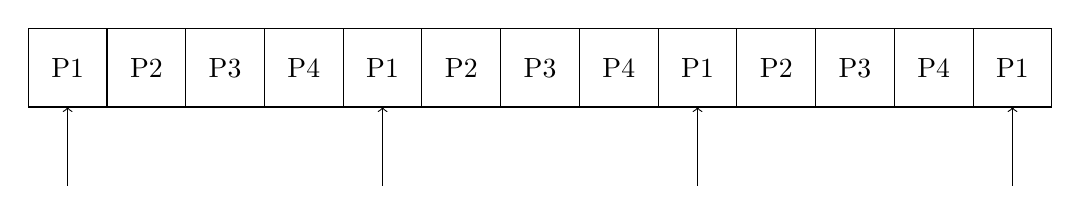
\begin{tikzpicture}
  \draw[step=1cm] (0,0) grid (13,1);
  \foreach \i in {0,4,8,12} {
    \draw (\i+.5,.5) node {P1};
  }
  \foreach \i in {0,4,8} {
    \draw (\i+1.5,.5) node {P2};
    \draw (\i+2.5,.5) node {P3};
    \draw (\i+3.5,.5) node {P4};
  }

  \foreach \i in {0,4,8,12} {
    \draw<3->[->] (\i+.5,-1) -- (\i+.5,0);
  }
\end{tikzpicture}
\end{adjustbox}

\begin{itemize}
  \item<4-> The \mintinline{fortran}|property1| values are gathered into a vector register.
  \item<5-> After the computation, the results are scattered back into memory.
  \item<6-> A cache line is 64 bytes, so only the first two values are on the first cache line.
  \item<6-> Must read two cache lines to fill the vector up.
\end{itemize}
\end{frame}

%-------------------------------------------------------------------------------
\begin{frame}[fragile]
\frametitle{Structure of arrays}
Switch type around to have an array per property.
\begin{minted}[frame=single,linenos,fontsize=\small]{fortran}
type grid
  real(kind=8), allocatable :: property1(:,:)
  real(kind=8), allocatable :: property2(:,:)
  real(kind=8), allocatable :: property3(:,:)
  real(kind=8), allocatable :: property4(:,:)
end type

do j = 1, ny
  do i = 1, nx
    grid%property1(i,j) = update_1()
    grid%property2(i,j) = update_2()
    grid%property3(i,j) = update_3()
    grid%property4(i,j) = update_4()
  end do
end do
\end{minted}
\end{frame}

%-------------------------------------------------------------------------------
\begin{frame}
\frametitle{Structure of arrays}
\begin{itemize}
  \item Order of data in memory has changed.
  \item<2-> What happens when we vectorise?
\end{itemize}

\begin{adjustbox}{max width={\textwidth}}
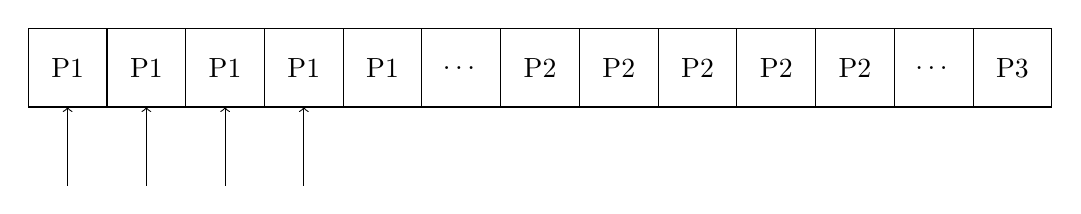
\begin{tikzpicture}
  \draw[step=1cm] (0,0) grid (13,1);
  \foreach \i in {0,...,4} {
    \draw (\i+.5,.5) node {P1};
  }
  \draw (5.5,.5) node {\dots};

  \foreach \i in {5,...,9} {
    \draw (\i+1.5,.5) node {P2};
  }
  \draw (11.5,.5) node {\dots};

  \foreach \i in {10} {
    \draw (\i+2.5,.5) node {P3};
  }

  \foreach \i in {0,...,3} {
    \draw<3->[->] (\i+.5,-1) -- (\i+.5,0);
  }
\end{tikzpicture}
\end{adjustbox}

\onslide<4->{
\begin{itemize}
  \item Coalesced memory accesses are key for high performance code.
  \item Adjacent vector lanes read adjacent memory locations.
  \item A cache line is 64 bytes, so can fill the vector from a single cache line.
  \item More efficient vectorisation.
\end{itemize}
}
\end{frame}

%-------------------------------------------------------------------------------
\section{Memory access patterns}
\begin{frame}[fragile]
\frametitle{Memory access patterns}
\begin{minted}{fortran}
do i = 1, N
  val = A(i)
end do
\end{minted}
\begin{adjustbox}{max width={\textwidth}}
\begin{tikzpicture}
  \draw[step=1cm] (-3,0) grid (11,1);
  \draw[dashed] (0,-.5) -- (0,1.5);
  \draw[dashed] (8,-.5) -- (8,1.5);
  \draw (0,-1) node {64 byte boundary};
  \foreach \i in {0,...,7} {
    \draw[->] (\i+.5,2) -- (\i+.5,1.2);
  }
\end{tikzpicture}
\end{adjustbox}
\begin{itemize}
  \item Ideal memory access pattern.
  \item All access is coalesced.
  \item Vectors are aligned to cache line boundary.
\end{itemize}
\end{frame}

%-------------------------------------------------------------------------------
\begin{frame}[fragile]
\frametitle{Memory access patterns}
\begin{minted}{fortran}
do i = 1, N
  val = A(i+3)
end do
\end{minted}
\begin{adjustbox}{max width={\textwidth}}
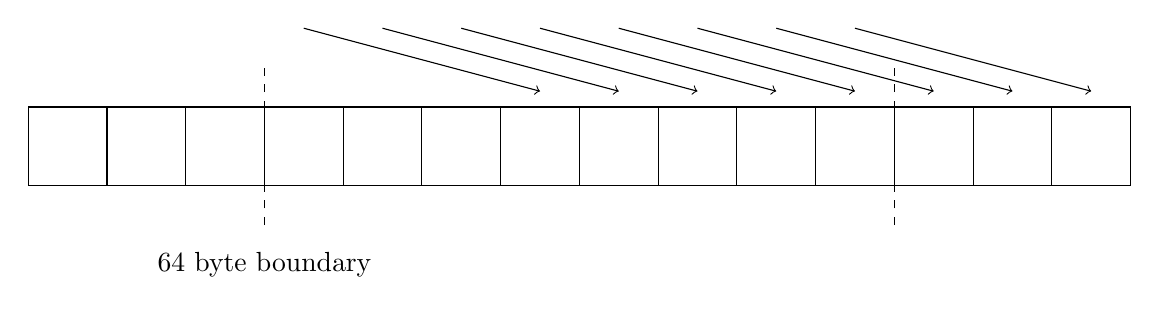
\begin{tikzpicture}
  \draw[step=1cm] (-3,0) grid (11,1);
  \draw[dashed] (0,-.5) -- (0,1.5);
  \draw[dashed] (8,-.5) -- (8,1.5);
  \draw (0,-1) node {64 byte boundary};
  \foreach \i in {0,...,7} {
    \draw[->] (\i+.5,2) -- (3+\i+.5,1.2);
  }
\end{tikzpicture}
\end{adjustbox}
\begin{itemize}
  \item OK memory access pattern.
  \item All access is coalesced, but split across cache lines.
  \item Still get good use of cache lines, but not as efficient as aligned version.
\end{itemize}
\end{frame}

%-------------------------------------------------------------------------------
\begin{frame}[fragile]
\frametitle{Memory access patterns}
\begin{minted}{fortran}
do i = 1, N
  val = A(j,i) ! equiv. A(j+3*i)
end do
\end{minted}
\begin{adjustbox}{max width={\textwidth}}
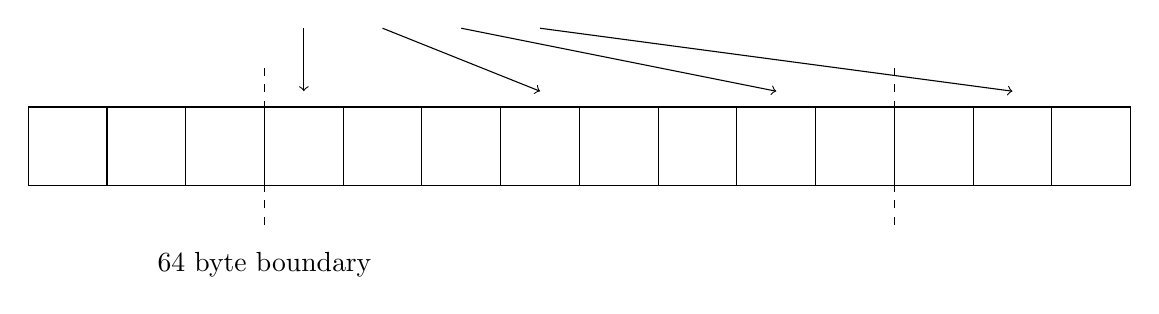
\begin{tikzpicture}
  \draw[step=1cm] (-3,0) grid (11,1);
  \draw[dashed] (0,-.5) -- (0,1.5);
  \draw[dashed] (8,-.5) -- (8,1.5);
  \draw (0,-1) node {64 byte boundary};
  \foreach \i in {0,...,3} {
    \draw[->] (\i+.5,2) -- (3*\i+.5,1.2);
  }
\end{tikzpicture}
\end{adjustbox}
\begin{itemize}
  \item Strided access results in multiple memory transactions.
  \item Kills throughput due to poor reuse of cached data.
  \item Very easy to fall into this trap with multi-dimensional arrays.
  \item Check your strides!
\end{itemize}
\end{frame}

%-------------------------------------------------------------------------------
\begin{frame}[fragile]
\frametitle{Memory access patterns}
\begin{minted}{fortran}
do i = 1, N
  val = A(B(i))
end do
\end{minted}
\begin{adjustbox}{max width={\textwidth}}
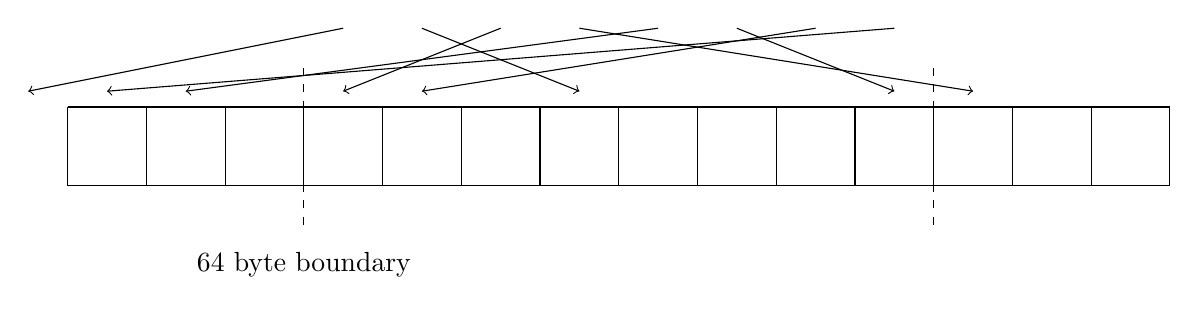
\begin{tikzpicture}
  \draw[step=1cm] (-3,0) grid (11,1);
  \draw[dashed] (0,-.5) -- (0,1.5);
  \draw[dashed] (8,-.5) -- (8,1.5);
  \draw (0,-1) node {64 byte boundary};
  \draw[->] (0.5,2) -- (-3.5,1.2);
  \draw[->] (1.5,2) -- (3.5,1.2);
  \draw[->] (2.5,2) -- (0.5,1.2);
  \draw[->] (3.5,2) -- (8.5,1.2);
  \draw[->] (4.5,2) -- (-1.5,1.2);
  \draw[->] (5.5,2) -- (7.5,1.2);
  \draw[->] (6.5,2) -- (1.5,1.2);
  \draw[->] (7.5,2) -- (-2.5,1.2);
\end{tikzpicture}
\end{adjustbox}
\begin{itemize}
  \item Essentially random access to memory.
  \item Little reuse of cache lines.
  \item Unpredictable pattern, so hardware prefetchers won't work efficiently.
  \item Very challenging!
\end{itemize}
\end{frame}

%-------------------------------------------------------------------------------
\section{NUMA}
\begin{frame}
\frametitle{NUMA Architecture}

Recall this cartoon of a dual-socket, shared memory system:
\begin{center}
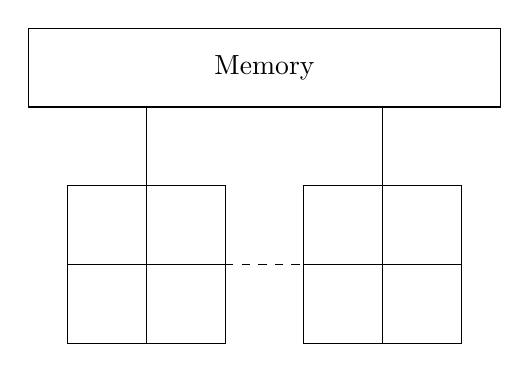
\begin{tikzpicture}
  % Draw 4 cores for socket 0
  \draw (0,0) rectangle (1,1);
  \draw (1,0) rectangle (2,1);
  \draw (0,1) rectangle (1,2);
  \draw (1,1) rectangle (2,2);

  % Draw 4 cores for socket 1
  \draw (3,0) rectangle (4,1);
  \draw (4,0) rectangle (5,1);
  \draw (3,1) rectangle (4,2);
  \draw (4,1) rectangle (5,2);

  % Draw large memory
  \draw (-0.5,3) rectangle (5.5,4);
  \draw (2.5,3.5) node {Memory};

  % Connect sockets to memory
  \draw (1,2) -- (1,3);
  \draw (4,2) -- (4,3);
  \draw[dashed] (2,1) -- (3,1); % QPI

\end{tikzpicture}
\end{center}

\emph{All} threads (each running on a core) can access the same memory.

\end{frame}
%-------------------------------------------------------------------------------

\begin{frame}
\frametitle{NUMA Architecture}
\begin{itemize}
  \item In reality on a dual-socket system each \emph{socket} is physically connected to half of the memory.
  \item Still shared memory: all cores can access all the memory.
  \item A core in the first socket wanting memory attached to the other socket must:
    \begin{itemize}
      \item Go via the socket-to-socket interconnect.
      \item Access memory via the other socket's memory controllers.
    \end{itemize}
  \item Accessing memory from other socket is slower than access from own socket.
\end{itemize}
\begin{center}
\resizebox{!}{3.5cm}{
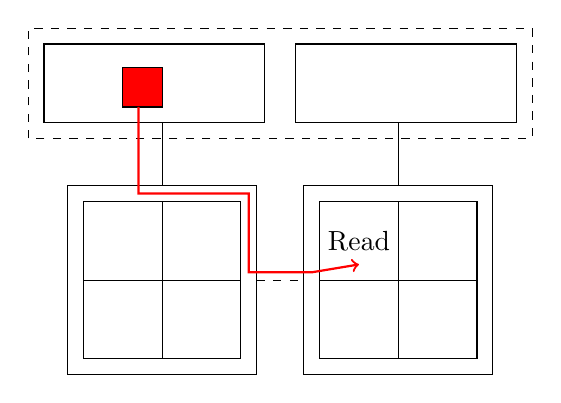
\begin{tikzpicture}
  % Draw 4 cores for socket 0
  \foreach \i in {0,1,3,4} {
    \foreach \j in {0, 1} {
      \draw (\i,\j) rectangle (\i+1,\j+1);
    }
  }

  % Draw sockets around cores
  \draw (-0.2, -0.2) rectangle (2.2, 2.2);
  \draw (2.8, -0.2) rectangle (5.2, 2.2);

  % Draw large memory
  \draw (-0.5,3) rectangle (2.3,4);
  \draw (2.7,3) rectangle (5.5,4);
  \draw[dashed] (-0.7,2.8) rectangle (5.7,4.2);

  % Connect sockets to memory
  \draw (1,2.2) -- (1,3);
  \draw (4,2.2) -- (4,3);
  \draw[dashed] (2.2,1) -- (2.8,1); % QPI

  % Show memory shared
  \pause
  \draw[fill=red] (0.5,3.2) rectangle (1,3.7);
  \draw (3.5,1.5) node {Read};
  \pause
  \draw[->,red,thick] (0.7,3.2) -- (0.7,2.1) -- (2.1,2.1) -- (2.1,1.1) -- (2.9,1.1) -- (3.5,1.2);

\end{tikzpicture}
}
\end{center}
\end{frame}

%-------------------------------------------------------------------------------
\begin{frame}
\frametitle{Memory allocation}
\begin{itemize}
  \item What happens when you run \mintinline{fortran}|allocate(A(1:N))|?
  \pause
  \item Allocating memory does not necessarily allocate memory!
  \item Memory is allocated when it's first used (i.e. \mintinline{fortran}|A(i) = 1.0|), one \emph{page} at a time.
  \item OS tends to use a \emph{first touch policy}.
  \item Memory is allocated in the closest NUMA region to the thread that first touches the data.
  \item Ideally want threads to use data in local NUMA region to reduce socket-to-socket interconnect transfers.
\end{itemize}
\end{frame}

%-------------------------------------------------------------------------------
\subsection{First touch}
\begin{frame}[fragile]
\frametitle{Taking advantage of first touch}
Parallelising your data initialisation routine might mean your main loops go faster!


\begin{minted}[fontsize=\small,linenos,frame=single]{fortran}
! Allocate and initialise vectors
allocate(A(N), B(N), C(N))
!$omp parallel do
do i = 1, N
  A(i) = 1.0
  B(i) = 2.0
  C(i) = 0.0
end do
!$omp end parallel do

! Vector add
!$omp parallel do
do i = 1, N
  C(i) = A(i) + B(i)
end do
!$omp end parallel do
\end{minted}

\end{frame}

%-------------------------------------------------------------------------------
\begin{frame}
\frametitle{NUMA-aware}
\begin{itemize}
  \item Parallelise your initialisation routines the same way you parallelise the main loops.
  \item This means each thread touches the same data in initialisation and compute.
  \item Should reduce the number of remote memory accesses needed and improve run times.
  \item But, OS is allowed to move threads around cores, and between sockets.
  \item This will mess up your NUMA aware code!
\end{itemize}
\end{frame}

%-------------------------------------------------------------------------------
\section{Thread affinity}
\begin{frame}
\frametitle{Pinning threads}
\begin{itemize}
  \item OpenMP gives you the controls to pin threads to specific cores.
  \item Exposed as \emph{places} and \emph{thread pinning policy} to those places.
  \item By default there is one place consisting of all the cores.
  \item Use the \mintinline{bash}|OMP_PROC_BIND| environment variable to set pinning for all \mintinline{fortran}|parallel| regions.
  \item Can use the \mintinline{bash}|proc_bind| clause for control of specific regions, but advise against this.
\end{itemize}
\end{frame}

%-------------------------------------------------------------------------------
\begin{frame}
\frametitle{OMP\_PROC\_BIND}
\begin{itemize}
  \item \mintinline{bash}|OMP_PROC_BIND=false|: Often the default; threads may move! \mintinline{fortran}|proc_bind| clauses ignored.
  \item \mintinline{bash}|OMP_PROC_BIND=true|: Threads won't move, and follow \mintinline{fortran}|proc_bind| clauses or else the implementation default pinning.
  \item \mintinline{bash}|OMP_PROC_BIND=master|: Threads pinned to same place as master thread.
  \item \mintinline{bash}|OMP_PROC_BIND=close|: Threads are assigned to places close to the master thread.
  If \mintinline{bash}|OMP_NUM_THREADS.eq.ncores|: thread 0 will pin to core 0; thread 1 will pin to core 1; etc
  \item \mintinline{bash}|OMP_PROC_BIND=spread|: Threads are assigned to places ``sparsely''.
  If \mintinline{bash}|OMP_NUM_THREADS.eq.ncores|: thread 0 will pin to socket 0 core 0; thread 1 will pin to socket 1 core 0; thread 2 will pin to socket 0 core 1; etc.
\end{itemize}
\end{frame}

%-------------------------------------------------------------------------------
\begin{frame}
\frametitle{Places}
\begin{itemize}
  \item The affinity (policy) defines how threads are assigned to places.
  \item Places allow you to divide up the hardware resource, so that threads can be assigned to them.
  \item Default: one place with all cores.
  \item Use \mintinline{bash}|OMP_PLACES| environment variable to control.
  \item \mintinline{bash}|OMP_PLACES=threads|: each place is a single hardware thread.
  \item \mintinline{bash}|OMP_PLACES=cores|: each place is a single core (containing one or more hardware threads).
  \item \mintinline{bash}|OMP_PLACES=sockets|: each place contains the cores of a single socket.
  \item Can also use list notation: \mintinline{bash}|OMP_PLACES="{0:4},{4:4},{8:4},{12:4}"|
\end{itemize}
\end{frame}

%-------------------------------------------------------------------------------
\begin{frame}
\frametitle{Thread pinning summary}
\begin{itemize}
  \item In general, going to want to just use \mintinline{bash}|OMP_PROC_BIND=true|.
  \item Sometimes \mintinline{bash}|spread| or \mintinline{bash}|close| gets better performance.
  \item Pinning rules can get complicated when there are multiple places, so prefer to use the predefined values.
  \item Most effective with a NUMA-aware implementation.
  \item Also helps reduce run-to-run timing variability.
  \item But must be careful with MPI+OpenMP pinning.
\end{itemize}
\end{frame}

%-------------------------------------------------------------------------------
\section{Hybrid MPI and OpenMP}
\begin{frame}
\frametitle{Why combine MPI+OpenMP}
\begin{itemize}
  \item Supercomputers are often constructed with a hierarchical structure:
    \begin{itemize}
      \item Shared memory nodes connected with a network.
    \end{itemize}
  \item Need MPI (or similar) to communicate between distributed nodes.
  \item With multi-core, could just run MPI everywhere (flat MPI).
  \item But there are advantages to running \emph{hybrid} MPI and OpenMP:
    \begin{itemize}
      \item Larger fewer messages to take advantage of network bandwidth.
      \item Fewer MPI ranks to manage (fewer to synchronise and for collectives).
      \item Can avoid memory copies for intra-node communication.
      \item Reduced memory footprint.
      \item Parallelise other problem dimensions not decomposed with MPI.
    \end{itemize}
\end{itemize}
\end{frame}

%-------------------------------------------------------------------------------
\begin{frame}
  \frametitle{Thread support levels}
  \begin{itemize}
    \item \mintinline{fortran}|MPI_THREAD_SINGLE| \\
    Only one thread will execute (no threads allowed).
  
    \item \mintinline{fortran}|MPI_THREAD_FUNNELED| \\
    May spawn threads, but only the original process may call MPI routines: the one that called \mintinline{fortran}|MPI_Init|.
  
    \item \mintinline{fortran}|MPI_THREAD_SERIALIZED| \\
    May spawn threads and any thread can make MPI calls, but only one at a time. \emph{Your} responsibility to synchronise.
  
    \item \mintinline{fortran}|MPI_THREAD_MULTIPLE| \\
    May spawn threads and any thread can make MPI calls. The MPI library has to deal with being called in parallel.
  \end{itemize}
  
  Remember to make sure ranks still match the MPI communications to avoid deadlock.
  
  \end{frame}

%-------------------------------------------------------------------------------
\section{Exercise}
\begin{frame}
\frametitle{Exercise}
\begin{itemize}
  \item Take your parallel 5-point stencil code and optimise it.
  \item Think about:
    \begin{itemize}
      \item Memory access patterns
      \item Vectorisation
      \item NUMA
    \end{itemize}
  \item Note down the performance differences your optimisations make.
  \item Calculate the achieved memory bandwidth of your stencil code.
  \item Extension: consider these optimisaions for the Jacobi solver.
\end{itemize}
\end{frame}

\end{document}
